\documentclass[12pt]{article}

\usepackage[T1]{fontenc}
\usepackage[a4paper, margin=1.5cm]{geometry}
\usepackage[colorlinks, urlcolor=blue, citecolor=red]{hyperref}
\usepackage[utf8]{inputenc}
\usepackage{amsmath, amsfonts, booktabs, enumitem, parskip, siunitx, tikz-qtree}

\usetikzlibrary{decorations.pathreplacing}

\newcommand{\euler}{\mathrm{e}}

\begin{document}

\textsc{Graduate Program in Computer Science,
  Universidade Federal de Santa Catarina} \\
\textsc{INE410104 (Design and Analysis of Algorithms)}

\textsc{Solutions to the 1\textsuperscript{st} Set of Exercises} \\
\textsc{Gustavo Zambonin, Matheus S. P. Bittencourt}

\section{Answers}

\begin{enumerate}
    \item 
    \begin{enumerate}
        \item Let the functions that represent the time complexities of algorithms $A$ and $B$ be $f(n) = n^{3}$ and $g(n) = 128n^{2}$, respectively, with $n \in \mathbb{N}$. Further, consider $t(n) = \frac{f(n)}{g(n)} \Rightarrow \frac{n}{128}$. By the ratio $t(n)$, algorithm $B$ is faster than $A$ when $n > 128$.
        \item Let the old and new computers be named $N_{1}$ and $N_{2}$, respectively, and $f(n) = 2^{n}$. The equations $t_{1} = \frac{2^{n_{1}}}{s}, t_{2} = \frac{2^{n_{2}}}{20s}$ give the time spent to solve an instance of $f(n)$ on $N_{1}$ and $N_{2}$ with $s$ instructions, with input sizes of $n_{1}$ and $n_{2}$. By setting $t_{1} = t_{2}$, it is possible to figure out that the twenty-fold increase in the number of instructions does not help too much in solving $f(n)$.
        \begin{align*}
            \tfrac{2^{n_{1}}}{s} = \tfrac{2^{n_{2}}}{20s} \\
            2^{n_{2}} = 20 \cdot 2^{N_{1}} \\
            n_{2} = n_{1} + \log_{2} 20 \\
            n_{2} \approx n_{1} + 4.32.
        \end{align*}
        It is evident that the new input size had a modest growth. Indeed, the new computer will run slower if $n > 4$. This is due to the fact that the complexity of $f(n)$ grows exponentially, while in this case, the computational power grew linearly. Ergo, one cannot execute $f(2n)$ and expect comparable results on $N_{2}$, since $n_{2} \ll 2 n_{1}$.
        
        % \item Let $t_1 = \frac{2^n}{s}$ be the running time for the old computer and $t_2 = \frac{2^{2n}}{20s}$ for the new one, with $s$ being the number of instructions that the old computer executes per minute. Let's compare the running times with the new computer solving an instance of the problem twice as large as the one being executed by the old one.
        % \begin{align*}
        %     r &= \frac{t_1}{t_2} \\
        %     &= \frac{2^n}{s}\frac{20s}{2^{2n}} \\
        %     &= \frac{20}{2^n}
        % \end{align*}
        % $r$ actually represents the speed up of the new computer, with a larger instance of the problem. The new computer will run slower with $n > 4$. This is due to the fact that the complexity of the problem grows exponentially while the computational power grew linearly.
        
    \end{enumerate}
    \item 
    \begin{enumerate}
        \item Let $t_{1}, \dots, t_{7}$ be the number of seconds in each period of the header row and $s = 10^{10}$. The values in the table below represent approximately $n \leq f^{-1}(t_{i} s)$.
        \begin{table}[htbp]
            \renewcommand{\arraystretch}{1.2}
            \setlength{\tabcolsep}{7pt}
            \centering
            \tiny
            \begin{tabular}{l*{7}{r}}
                \toprule
                $f(n)$ / $t$ & 1 second & 1 minute & 1 hour & 1 day & 1 month & 1 year & 1 century \\ \midrule
                $\log_{2} n$ & $2^{\num{1.E+10}}$ & $2^{\num{6.E+11}}$ & $2^{\num{3.6E+13}}$ & $2^{\num{8.64E+14}}$ & $2^{\num{2.592E+16}}$ & $2^{\num{3.11E+17}}$ & $2^{\num{3.11E+19}}$ \\
                $\sqrt{n}$ & $\num{1.E+20}$ & $\num{3.6E+23}$ & $\num{1.296E+27}$ & $\num{7.465E+29}$ & $\num{6.718E+32}$ & $\num{9.675E+34}$ & $\num{9.675E+38}$ \\
                $n$ & $\num{1.E+10}$ & $\num{6.E+11}$ & $\num{3.6E+13}$ & $\num{8.64E+14}$ & $\num{2.592E+16}$ & $\num{3.11E+17}$ & $\num{3.11E+19}$ \\
                $n \log_{2} n$ & $\num{3.522E+08}$ & $\num{1.763E+10}$ & $\num{9.063E+11}$ & $\num{1.957E+13}$ & $\num{5.299E+14}$ & $\num{5.936E+15}$ & $\num{5.283E+17}$ \\
                $n^{2}$ & $\num{1.E+05}$ & $\num{7.746E+05}$ & $\num{6.E+06}$ & $\num{2.939E+07}$ & $\num{1.61E+08}$ & $\num{5.577E+08}$ & $\num{5.577E+09}$ \\
                $n^{3}$ & $\num{2.154E+03}$ & $\num{8.434E+03}$ & $\num{3.302E+04}$ & $\num{9.524E+04}$ & $\num{2.959E+05}$ & $\num{6.775E+05}$ & $\num{3.145E+06}$ \\
                $2^{n}$ & $\num{3.322E+01}$ & $\num{3.913E+01}$ & $\num{4.503E+01}$ & $\num{4.962E+01}$ & $\num{5.452E+01}$ & $\num{5.811E+01}$ & $\num{6.475E+01}$ \\
                $n!$ & $\num{1.3E+01}$ & $\num{1.5E+01}$ & $\num{1.6E+01}$ & $\num{1.7E+01}$ & $\num{1.8E+01}$ & $\num{1.9E+01}$ & $\num{2.1E+01}$ \\
                \bottomrule
            \end{tabular}
        \end{table}
        % TODO
        \item The ``find-min'' operation is fastest on the binary and Fibonacci heaps, since it is constant. The ``delete-min'' operation should be fastest on the Fibonacci heap, since an $\mathcal{O}(\log n)$ time complexity represents an amortised asymptotic upper bound, whereas the other heaps' $\Theta(\log n)$ is tight. Indeed, given a worst case scenario, both operations take exactly the same time to complete, but otherwise the Fibonacci heap does not take $\log n$ steps to finish the operation in average. The ``insert'' operation is fastest on the binomial and Fibonacci heaps. Thus, the Fibonacci heap is overall the fastest data structure when compared to binary and binomial heaps.
        \item
        \begin{enumerate}
            % TODO log, lg, ln?
            \item $(\ln n)^{\ln n} \in \Omega(\frac{n}{\ln n})$, for $n_{0} > 7$ and $c = 1$.
            \item $n^{2} \in \Omega(n^{\frac{1}{2}})$, for $n_{0} > 1$ and $c = 1$.
            \item $n! \in \Omega(n^{n - 47})$, for $n_{0} > 1$ and $c = 1$.
            \item $2^{{(\ln n)}^{2}} \in \Omega((\ln n)^{\ln n})$, for $n_{0} > 1$ and $c = 1$.
            \item $n^{2} \in \Theta(n + n^{2})$, for $n_{0} > 1, c_{1} = \frac{1}{2}$ and $c_{2} = 1$.
            \item $n + (\ln n)^{2} \in \Theta(10n + \ln n)$, for $n_{0} > \frac{1}{2}, c_{1} = \frac{1}{2}$ and $c_{2} = 1$.
            \item $\ln 2n \in \Theta(\ln 3n)$, for $n_{0} > 1, c_{1} = \frac{1}{2}$ and $c_{2} = 1$.
            \item $n (\ln n)^{2} \in \mathcal{O}(\frac{n^{2}}{\ln n})$, for $n_{0} > 7$ and $c = 1$.
        \end{enumerate}
    \end{enumerate}
    \item
    \begin{enumerate}
        \item Let $P(n) = \sum_{i = 1}^{n} i = \frac{n (n + 1)}{2}$. $P(1)$ holds, since $\frac{1 (1 + 1)}{2} = 1$. The inductive step is proved below, using the hypothesis that $P(k)$ is true.
        \begin{align*}
            P(k) + (k + 1) &\stackrel{?}{=} P(k + 1) \\
            \frac{k (k + 1)}{2} + (k + 1) &\stackrel{?}{=} \\
            \frac{k (k + 1) + 2(k + 1)}{2} &\stackrel{?}{=} \\
            \frac{(k + 1)(k + 2)}{2} &\stackrel{?}{=} \\
            \frac{(k + 1)((k + 1) + 1)}{2} &= P(k + 1).
        \end{align*}
        \item Let $P(n) = \sum_{i = 0}^{n} i^{2} = \frac{n (n + 1) (2n + 1)}{6}$. $P(0)$ holds, since $\frac{0 (0 + 1) (2 \cdot 0 + 1)}{2} = 0$. The inductive step is proved below, using the hypothesis that $P(k)$ is true.
        \begin{align*}
            P(k) + (k + 1)^{2} &\stackrel{?}{=} P(k + 1) \\
            \frac{k (k + 1) (2k + 1)}{6} + (k + 1)^{2} &\stackrel{?}{=} \\
            \frac{k (k + 1) (2k + 1) + 6(k + 1)^{2}}{6} &\stackrel{?}{=} \\
            \frac{(k + 1)(k(2k + 1) + 6(k + 1))}{6} &\stackrel{?}{=} \\
            \frac{(k + 1)(2k^2 + 7k + 6)}{6} &\stackrel{?}{=} P(k + 1) \\
            &\stackrel{?}{=} \frac{(k + 1)((k + 1) + 1)(2(k + 1) + 1)}{6} \\
            \frac{(k + 1)(2k^2 + 7k + 6)}{6} &= \frac{(k + 1)(k + 2)(2k + 3)}{6}.
        \end{align*}
        \item Let $P(n) = \sum_{i = 1}^{n} (2i - 1) = n^{2}$. $P(1)$ holds, since $2 \cdot 1 - 1 = 1^{2}$. The inductive step is proved below, using the hypothesis that $P(k)$ is true.
        \begin{align*}
            P(k) + 2(k + 1) - 1 &\stackrel{?}{=} P(k + 1) \\
            k^{2} + 2(k + 1) - 1 &\stackrel{?}{=} \\
            k^{2} + 2k + 1 &\stackrel{?}{=} \\
            (k + 1)^{2} &= P(k + 1).
        \end{align*}
        \item Let $P(n) = \sum_{i = 0}^{n} i^{3} = \frac{n^{2} (n + 1)^{2}}{4}$. $P(0)$ holds, since $\frac{0^{2} \cdot (0 + 0)^{2}}{4} = 0$. The inductive step is proved below, using the hypothesis that $P(k)$ is true.
        \begin{align*}
            P(k) + (k + 1)^{3} &\stackrel{?}{=} P(k + 1) \\
            \frac{k^{2} (k + 1)^{2}}{4} + (k + 1)^{3} &\stackrel{?}{=} \\
            \frac{k^{2} (k + 1)^{2} + 4(k + 1)^{3}}{4} &\stackrel{?}{=} \\
            \frac{(k^{2} + 4(k + 1))(k + 1)^{2}}{4} &\stackrel{?}{=} \\
            \frac{(k^{2} + 4k + 4)(k + 1)^{2}}{4} &\stackrel{?}{=} \\
            \frac{(k + 2)^{2}(k + 1)^{2}}{4} &= P(k + 1).
        \end{align*}
    \end{enumerate}
    \item
    \begin{enumerate}
        \item Let \[
            T(n) = \begin{cases}
                0 &\text{if } n = 1, \\
                T(n - 1) + c &\text{if } n > 1
            \end{cases}
        \] for any constant $c$. By the iteration method,
        \begin{align*}
            T(n) &= c + T(n - 1) \\
            &= c + c + T(n - 2) \\
            &= c + c + c + T(n - 3) \cdots \\
            &= ic + T(n - i).
        \end{align*}
        Consider $T(n - i) \Leftrightarrow T(1)$. Thus, $n - i = 1$ and $i = n - 1$, which gives
        \begin{align*}
            T(n) &= (n - 1)c + T(n - (n - 1)) \\
            &= nc - c + T(1) \\
            T(n) &\in \Theta(n).
        \end{align*}
        To prove the final formula by weak induction, let $T(n) = c(n - 1)$. $T(1)$ holds, since $c(1 - 1) = 0$. The inductive step is proved below, using the hypothesis that $T(n - 1)$ is true.
        \begin{align*}
            T(n - 1) + c &\stackrel{?}{=} T(n) \\
            c((n - 1) - 1) + c &\stackrel{?}{=} \\
            c(n - 2) + c(1) &\stackrel{?}{=} \\
            c(n - 1) &= T(n).
        \end{align*}
        \item Let \[
            T(n) = \begin{cases}
                0 &\text{if } n = 1, \\
                T(n - 1) + 2^{n} &\text{if } n > 1.
            \end{cases}
        \] By the iteration method,
        \begin{align*}
            T(n) &= 2^{n} + T(n - 1) \\
            &= 2^{n} + 2^{n - 1} + T(n - 2) \\
            &= 2^{n} + 2^{n - 1} + 2^{n - 2} + T(n - 3) \cdots \\
            &= \sum_{i = 2}^{n} 2^{i}.
        \end{align*}
        The sum of this geometric series is exactly $\frac{2^{n + 1} - 1}{2 - 1} - 2^{0} - 2^{1} = 2^{n + 1} - 4$, since $i$ does not start at $0$. To prove the final formula by weak induction, let $T(n) = 2^{n + 1} - 4$. $T(1)$ holds, since $2^{1 + 1} - 4 = 0$. The inductive step is proved below, using the hypothesis that $T(n - 1)$ is true.
        \begin{align*}
            T(n - 1) + 2^{n} &\stackrel{?}{=} T(n) \\
            2^{(n - 1) + 1} - 4 + 2^{n} &\stackrel{?}{=} \\
            2^{n + 1} - 4 &= T(n).
        \end{align*}
        \item\label{ex:4c} Let \[
            T(n) = \begin{cases}
                k &\text{if } n = 0, \\
                cT(n - 1) &\text{if } n > 0,
            \end{cases}
        \] for any constants $c, k$. By the iteration method,
        \begin{align*}
            T(n) &= cT(n - 1) \\
            &= c(cT(n - 2)) \\
            &= c(c(cT(n - 3))) \cdots \\
            &= c^{i} T(n - i).
        \end{align*}
        Consider $T(n - i) \Leftrightarrow T(0)$. Thus, $n - i = 0$ and $i = n$, which gives
        \begin{align*}
            T(n) &= c^{n} T(n - n)  \\
            &= c^{n} k \\
            T(n) &\in \Theta(c^{n}).
        \end{align*}
        To prove the final formula by weak induction, let $T(n) = c^{n} k$. $T(0)$ holds, since $c^{0} k = k$. The inductive step is proved below, using the hypothesis that $T(n - 1)$ is true.
        \begin{align*}
            cT(n - 1) &\stackrel{?}{=} T(n) \\
            c c^{n - 1} k &\stackrel{?}{=} \\
            c^{n} k &= T(n). 
        \end{align*}
        \item\label{ex:4d} Let \[
            T(n) = \begin{cases}
                1 &\text{if } n = 1, \\
                3T(\frac{n}{2}) + n &\text{if } n > 1.
            \end{cases}
        \] By the iteration method,
        \begin{align*}
            T(n) &= n + 3T(\tfrac{n}{2}) \\
            &= n + 3(\tfrac{n}{2} + 3T(\tfrac{n}{4})) \\ 
            &= n + 3(\tfrac{n}{2} + 3(\tfrac{n}{4} + 3T(\tfrac{n}{8}))) \cdots \\
            &= n\sum_{i = 0}^{\log_{2} n} (\tfrac{3}{2})^{i} + 3^{\log_{2} n}.
        \end{align*}
        Recall that the last term is obtained as one reaches the very end of the iteration. Furthermore, the sum of this geometric series is exactly \[\left(\frac{\frac{3}{2}^{\log_{2} n + 1} - 1}{\frac{3}{2} - 1}\right) = 2(\tfrac{3}{2}^{\log_{2} n + 1} - 1).\]
        The closed formula is derived as follows.
        \begin{align*}
            T(n) &= 2n(\tfrac{3}{2}^{\log_{2} n + 1} - 1) + 3^{\log_{2} n} \\
            &= 2n(\tfrac{3}{2}^{\log_{2} n} \cdot \tfrac{3}{2} - 1) + n^{\log_{2} 3} \\
            &= \tfrac{6n}{2}\tfrac{3}{2}^{\log_{2} n} - 2n + n^{\log_{2} 3} \\
            &= 3nn^{\log_{2} \tfrac{3}{2}} - 2n + n^{\log_{2} 3} \\
            &= 3n^{\log_{2} 3 - 1 + 1} + n^{\log_{2} 3} - 2n \\
            &= 4n^{\log_{2} 3} - 2n \\
            T(n) &\in \Theta(\text{poly}(n)).
        \end{align*}
        To prove the final formula by weak induction, let $T(n) = 4n^{\log_{2} 3} - 2n$. $P(1)$ holds, since $3 \cdot 1^{\log_{2} 3} - 2 \cdot 1 = 1$. The inductive step is proved below, using the hypothesis that $T(\frac{n}{2})$ is true.
        \begin{align*}
            3T(\tfrac{n}{2}) + n &\stackrel{?}{=} T(n) \\
            3(4\tfrac{n}{2}^{\log_{2} 3} - \tfrac{2n}{2}) + n &\stackrel{?}{=} \\
            12\tfrac{n}{2}^{\log_{2} 3} - 2n &\stackrel{?}{=} \\
            12 \cdot 2^{-\log_2 3} \cdot n^{\log_2 3} - 2n &\stackrel{?}{=} \\
            4n^{\log_{2} 3} - 2n &= T(n).
        \end{align*}
    \end{enumerate}
    \item
    \begin{enumerate}
        \item Let $T(n) = T(\frac{n}{2}) + \Theta(1)$, with $a = 1, b = 2$ and $f(n) \in \Theta(1)$. Since $n^{\log_{2} 1} = 1$ and $f(n) \in \Theta(1)$, the second case may be applied. Thus, $T(n) \in \Theta(\log_{2} n)$.
        \item Let $T(n) = T(\frac{9n}{10}) + n$, with $a = 1, b = \frac{10}{9}$ and $f(n) = n$. It occurs that $n^{\log_{\frac{9}{10}} 1} = 1$, $f(n) \in \Omega(n^{\log_{\frac{10}{9}} 1 + \epsilon})$ and $\frac{9n}{10} \leq cn$ with \emph{e.g.} $\epsilon < 1$ and $c = \frac{10}{11}$. Thus, the third case may be applied, giving $T(n) \in \Theta(n)$.
        \item Let $T(n) = 16T(\frac{n}{4}) + n^{2}$, with $a = 16, b = 4$ and $f(n) = n^{2}$. Since $n^{\log_{4} 16} = n^{2}$ and $f(n) \in \Theta(n^{2})$, the second case may be applied. Thus, $T(n) \in \Theta(n^{2} \log_{2} n)$.
        \item Let $T(n) = 7T(\frac{n}{3}) + n^{2}$, with $a = 7, b = 3$ and $f(n) = n^{2}$. It occurs that $n^{\log_{3} 7} \approx n^{1.77}$, $f(n) \in \Omega(n^{1.77 + \epsilon})$ and $\frac{7n^{2}}{9} \leq cn^{2}$ with \emph{e.g.} $\epsilon < 2 - \log_3 7$ and $c = \frac{8}{9}$. Thus, the third case may be applied, giving $T(n) \in \Theta(n^{2})$.
    \end{enumerate}
    \item Dashed arrows represent the total cost of each level in the tree. Dotted edges mean the natural expansion of the subtrees. When applicable, the floor function is disregarded for simplicity.
    \begin{enumerate}
        \item Let $T(n) = 2T(\frac{n}{2}) + \Theta(n)$. By the recursion-tree method, $T(n) = n \log_{2} n + n$. Thus, $T(n) \in \Theta(n \log_2 n)$.
        \begin{figure}[htbp]
          \centering
          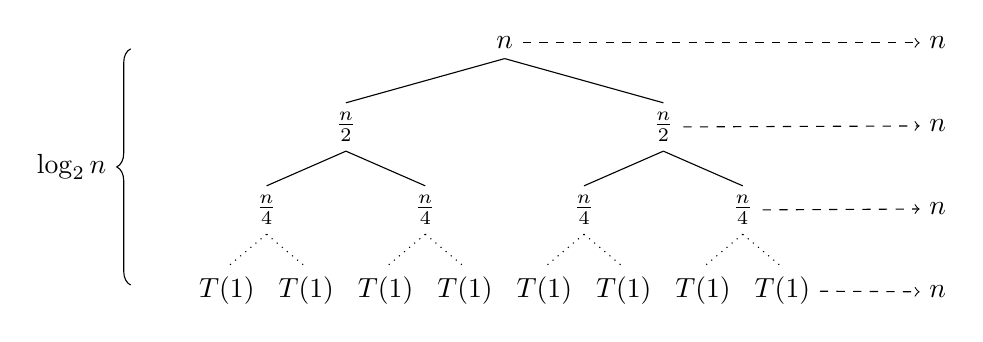
\begin{tikzpicture}
            \begin{scope}[xshift=-4.75cm]
              \draw [decorate,decoration={brace,amplitude=5pt}]
                (0, -3) -- (0, 0) node [black,midway,xshift=-0.75cm] {$\log_{2} n$};
            \end{scope}
            \begin{scope}
            \Tree
              [.\node(n0){$n$};
                [.\node{$\frac{n}{2}$};
                  [.{$\frac{n}{4}$}
                    \edge[dotted] node {}; $T(1)$
                    \edge[dotted] node {}; $T(1)$
                  ]
                  [.{$\frac{n}{4}$}
                    \edge[dotted] node {}; $T(1)$
                    \edge[dotted] node {}; $T(1)$
                  ]
                ]
                [.\node(n1){$\frac{n}{2}$};
                  [.{$\frac{n}{4}$}
                    \edge[dotted] node {}; $T(1)$
                    \edge[dotted] node {}; $T(1)$
                  ]
                  [.\node(n2){$\frac{n}{4}$};
                    \edge[dotted] node {}; $T(1)$
                    \edge[dotted] node {}; \node(n3){$T(1)$};
                  ]
                ]
              ]
            \end{scope}
              \begin{scope}[xshift=5.5cm]
            \tikzset{edge from parent/.append style={draw=none}}
            \Tree
              [.\node(c0){$n$};
                [.\node(c1){$n$};
                  [.\node(c2){$n$};
                    \node(c3){$n$};
                  ]
                ]
              ]
          \end{scope}
          \begin{scope}[->, dashed]
            \draw (n0) -- (c0);
            \draw (n1) -- (c1);
            \draw (n2) -- (c2);
            \draw (n3) -- (c3);
          \end{scope}
          \end{tikzpicture}
        \end{figure}
    \item Let $T(n) = 3T(\lfloor\frac{n}{2}\rfloor) + \Theta(n)$. By the recursion-tree method, $T(n) = n\sum_{i = 0}^{\log_{2} n} (\tfrac{3}{2})^{i} + n^{\log_{2} 3}$. As per Exercise~\ref{ex:4d}, $T(n) \in \Theta(\text{poly}(n))$.
        \begin{figure}[htbp]
          \centering
          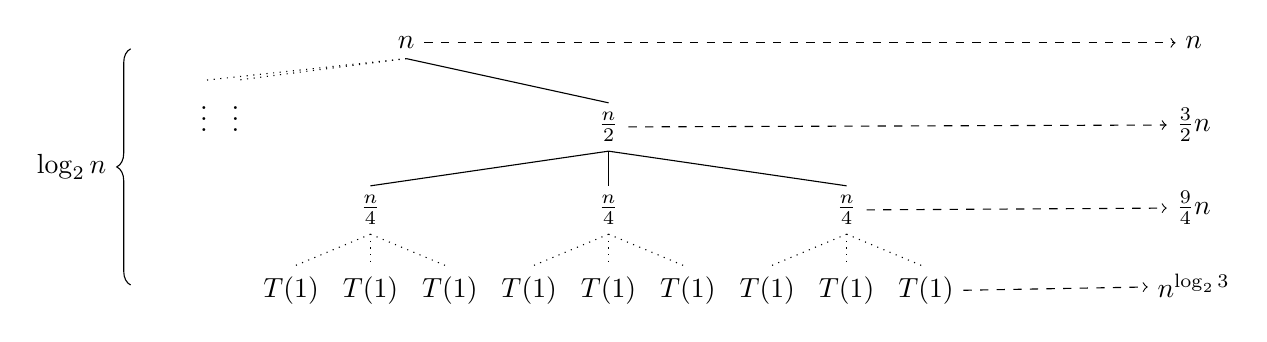
\begin{tikzpicture}
            \begin{scope}[xshift=-3.5cm]
              \draw [decorate,decoration={brace,amplitude=5pt}]
                (0, -3) -- (0, 0) node [black,midway,xshift=-0.75cm] {$\log_{2} n$};
            \end{scope}
            \begin{scope}
            \Tree
              [.\node(n0){$n$};
                \edge[dotted] node {}; $\vdots$
                \edge[dotted] node {}; $\vdots$
                [.\node(n1){$\frac{n}{2}$};
                  [.{$\frac{n}{4}$}
                    \edge[dotted] node {}; $T(1)$
                    \edge[dotted] node {}; $T(1)$
                    \edge[dotted] node {}; $T(1)$
                  ]
                  [.{$\frac{n}{4}$}
                    \edge[dotted] node {}; $T(1)$
                    \edge[dotted] node {}; $T(1)$
                    \edge[dotted] node {}; $T(1)$
                  ]
                  [.\node(n2){$\frac{n}{4}$};
                    \edge[dotted] node {}; $T(1)$
                    \edge[dotted] node {}; $T(1)$
                    \edge[dotted] node {}; \node(n3){$T(1)$};
                  ]
                ]
              ]
            \end{scope}
            \begin{scope}[xshift=10cm]
            \tikzset{edge from parent/.append style={draw=none}}
            \Tree
              [.\node(c0){$n$};
                [.\node(c1){$\frac{3}{2}n$};
                  [.\node(c2){$\frac{9}{4}n$};
                    \node(c3){$n^{\log_{2} 3}$};
                  ]
                ]
              ]
          \end{scope}
          \begin{scope}[->, dashed]
            \draw (n0) -- (c0);
            \draw (n1) -- (c1);
            \draw (n2) -- (c2);
            \draw (n3) -- (c3);
          \end{scope}
          \end{tikzpicture}
        \end{figure}
    \item Let $T(n) = 4T(\lfloor\frac{n}{2}\rfloor) + \Theta(n)$. By the recursion-tree method, $T(n) = n\sum_{i = 0}^{\log_{2} n} 2^{i} + n^{2} $. Using the sum of geometric series, $T(n) = n\frac{2^{\log_{2} n + 1} - 1}{2 - 1} + n^{2}$, which gives $n(2n - 1) + n^{2}$, and thus $T(n) \in \Theta(n^{2})$.
        \begin{figure}[htbp]
          \centering
          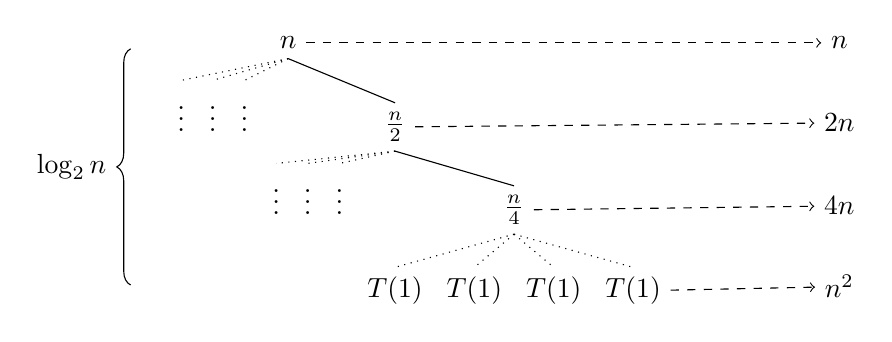
\begin{tikzpicture}
            \begin{scope}[xshift=-2cm]
              \draw [decorate,decoration={brace,amplitude=5pt}]
                (0, -3) -- (0, 0) node [black,midway,xshift=-0.75cm] {$\log_{2} n$};
            \end{scope}
            \begin{scope}
            \Tree
              [.\node(n0){$n$};
                \edge[dotted] node {}; $\vdots$
                \edge[dotted] node {}; $\vdots$
                \edge[dotted] node {}; $\vdots$
                [.\node(n1){$\frac{n}{2}$};
                  \edge[dotted] node {}; $\vdots$
                  \edge[dotted] node {}; $\vdots$
                  \edge[dotted] node {}; $\vdots$
                  [.\node(n2){$\frac{n}{4}$};
                    \edge[dotted] node {}; $T(1)$
                    \edge[dotted] node {}; $T(1)$
                    \edge[dotted] node {}; $T(1)$
                    \edge[dotted] node {}; \node(n3){$T(1)$};
                  ]
                ]
              ]
            \end{scope}
            \begin{scope}[xshift=7cm]
            \tikzset{edge from parent/.append style={draw=none}}
            \Tree
              [.\node(c0){$n$};
                [.\node(c1){$2n$};
                  [.\node(c2){$4n$};
                    \node(c3){$n^2$};
                  ]
                ]
              ]
          \end{scope}
          \begin{scope}[->, dashed]
            \draw (n0) -- (c0);
            \draw (n1) -- (c1);
            \draw (n2) -- (c2);
            \draw (n3) -- (c3);
          \end{scope}
          \end{tikzpicture}
        \end{figure}
    \item Let $T(n) = 2T(\frac{n}{2}) + \Theta(n^{2})$. By the recursion-tree method, $T(n) = n^{2} \sum_{i = 0}^{\log_{2} n} 2^{-i} + n$. Using the sum of geometric series, $T(n) = n^{2} \frac{2^{-(\log_{2} n + 1)} - 1}{\frac{1}{2} - 1} + n$, which gives $n^{2}(2 - \frac{1}{n}) + n$, and thus $T(n) \in \Theta(n^{2})$.
        \begin{figure}[htbp]
          \centering
          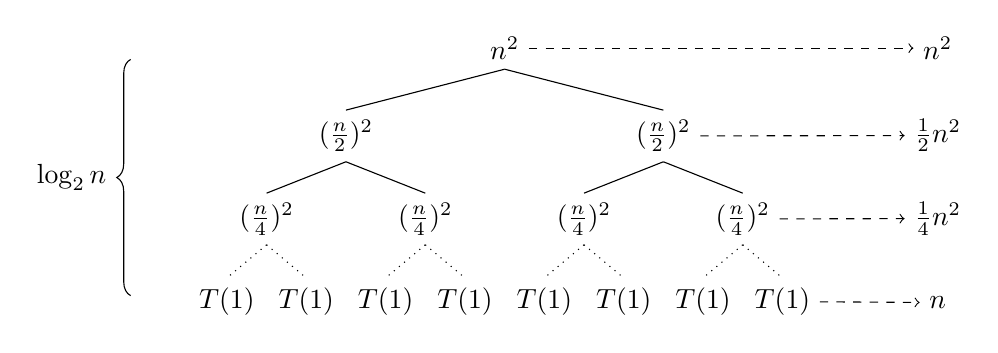
\begin{tikzpicture}
            \begin{scope}[xshift=-4.75cm]
              \draw [decorate,decoration={brace,amplitude=5pt}]
                (0, -3) -- (0, 0) node [black,midway,xshift=-0.75cm] {$\log_{2} n$};
            \end{scope}
            \begin{scope}
            \Tree
              [.\node(n0){$n^{2}$};
                [.\node{$(\frac{n}{2})^{2}$};
                  [.{$(\frac{n}{4})^{2}$}
                    \edge[dotted] node {}; $T(1)$
                    \edge[dotted] node {}; $T(1)$
                  ]
                  [.{$(\frac{n}{4})^{2}$}
                    \edge[dotted] node {}; $T(1)$
                    \edge[dotted] node {}; $T(1)$
                  ]
                ]
                [.\node(n1){$(\frac{n}{2})^{2}$};
                  [.{$(\frac{n}{4})^{2}$}
                    \edge[dotted] node {}; $T(1)$
                    \edge[dotted] node {}; $T(1)$
                  ]
                  [.\node(n2){$(\frac{n}{4})^{2}$};
                    \edge[dotted] node {}; $T(1)$
                    \edge[dotted] node {}; \node(n3){$T(1)$};
                  ]
                ]
              ]
            \end{scope}
              \begin{scope}[xshift=5.5cm]
            \tikzset{edge from parent/.append style={draw=none}}
            \Tree
              [.\node(c0){$n^{2}$};
                [.\node(c1){$\frac{1}{2}n^{2}$};
                  [.\node(c2){$\frac{1}{4}n^{2}$};
                    \node(c3){$n$};
                  ]
                ]
              ]
          \end{scope}
          \begin{scope}[->, dashed]
            \draw (n0) -- (c0);
            \draw (n1) -- (c1);
            \draw (n2) -- (c2);
            \draw (n3) -- (c3);
          \end{scope}
          \end{tikzpicture}
        \end{figure}
    \item Let $T(n) = 2T(\frac{n}{3}) + \Theta(n)$. By the recursion-tree method, $T(n) = n\sum_{i = 0}^{\log_{3} n} (\frac{2}{3})^{i} + 2^{\log_{3} n}$. Using the sum of geometric series, 
    \begin{align*}
        T(n) &= n \frac{\frac{2}{3}^{\log_{3} n + 1} - 1}{\frac{2}{3} - 1} + 2^{\log_{3} n} \\
        &= -3n (\tfrac{2}{3} \cdot \tfrac{2}{3}^{\log_{3} n} - 1) + 2^{\log_{3} n} \\
        &= -3n (\tfrac{2}{3} \cdot n^{\log_{3} \tfrac{2}{3}} - 1) + n^{\log_{3} 2} \\
        &= -3n (\tfrac{2}{3} \cdot n^{\log_{3} 2 - 1} - 1) + n^{\log_{3} 2} \\
        &= -2n^{\log_{3} 2} + 3n + n^{\log_{3} 2} \\
        &= -n^{\log_{3} 2} + 3n \\
        T(n) &\in \Theta(n).
    \end{align*}
        \begin{figure}[htbp]
          \centering
          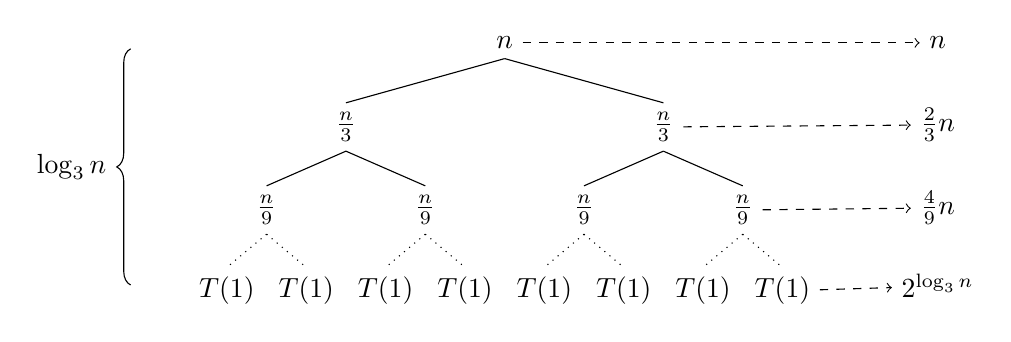
\begin{tikzpicture}
            \begin{scope}[xshift=-4.75cm]
              \draw [decorate,decoration={brace,amplitude=5pt}]
                (0, -3) -- (0, 0) node [black,midway,xshift=-0.75cm] {$\log_{3} n$};
            \end{scope}
            \begin{scope}
            \Tree
              [.\node(n0){$n$};
                [.\node{$\frac{n}{3}$};
                  [.{$\frac{n}{9}$}
                    \edge[dotted] node {}; $T(1)$
                    \edge[dotted] node {}; $T(1)$
                  ]
                  [.{$\frac{n}{9}$}
                    \edge[dotted] node {}; $T(1)$
                    \edge[dotted] node {}; $T(1)$
                  ]
                ]
                [.\node(n1){$\frac{n}{3}$};
                  [.{$\frac{n}{9}$}
                    \edge[dotted] node {}; $T(1)$
                    \edge[dotted] node {}; $T(1)$
                  ]
                  [.\node(n2){$\frac{n}{9}$};
                    \edge[dotted] node {}; $T(1)$
                    \edge[dotted] node {}; \node(n3){$T(1)$};
                  ]
                ]
              ]
            \end{scope}
              \begin{scope}[xshift=5.5cm]
            \tikzset{edge from parent/.append style={draw=none}}
            \Tree
              [.\node(c0){$n$};
                [.\node(c1){$\frac{2}{3}n$};
                  [.\node(c2){$\frac{4}{9}n$};
                    \node(c3){$2^{\log_{3} n}$};
                  ]
                ]
              ]
          \end{scope}
          \begin{scope}[->, dashed]
            \draw (n0) -- (c0);
            \draw (n1) -- (c1);
            \draw (n2) -- (c2);
            \draw (n3) -- (c3);
          \end{scope}
          \end{tikzpicture}
        \end{figure}
    \end{enumerate}
    \item As per the analysis presented below, the most efficient algorithm is~\ref{ex:7c}, with a quasilinear time complexity.
    \begin{enumerate}
        \item Let $T(n) = 5T(\frac{n}{2}) + \mathcal{O}(n)$. By the master method, $a = 5, b = 2$ and $f(n) \in \mathcal{O}(n)$. It occurs that $n^{\log_{2} 5} \approx n^{2.32}$, $f(n) \in \mathcal{O}(n^{2.32 - \epsilon})$ with \emph{e.g.} $\epsilon > \log_{2} 5 - 1$. Thus, the first case may be applied, giving $T(n) \in \Theta(n^{\log_{2} 5})$.
        \item Let $T(n) = 2T(n - 1) + \mathcal{O}(1)$. The recurrence is a special case of Exercise~\ref{ex:4c}, thus giving $T(n) \in \Theta(2^{n})$.
        \item\label{ex:7c} Let $T(n) = 9T(\frac{n}{3}) + \mathcal{O}(n^{2})$. By the master method, $a = 9, b = 3$ and $f(n) \in \mathcal{O}(n^{2})$. Since $n^{\log_{3} 9} = n^{2}$ and $f(n) \in \Theta(n^{2})$, the second case may be applied. Thus, $T(n) \in \Theta(n^{2} \log_{2} n)$.
    \end{enumerate}
\end{enumerate}

\appendix

\section{Rationale for Q2a}

Define $t_{1}, \dots, t_{7}$ and $s = 10^{10}$ as above. The equation $t_{i} = \frac{f(n)}{s}$, or its simpler form $n = f^{-1}(t_{i} s)$, has to be solved in order to find out the maximum $n$ allowed to execute for a period of time using $f(n)$. Deducing $f^{-1}$ is not trivial for some of the rows. In the case of $n \log_{2} n = c$ for some constant $c$, the Lambert $W$-function is used:
\begin{align*}
    n \log_{2} n &= c \\
    n \ln n &= c \ln 2 \\
    \euler^{\ln n} \ln n &= c \ln 2 \\
    \ln n &= W(c \ln 2) \\
    n &= \euler^{W(c \ln 2)}.
\end{align*}
Moreover, to invert the factorial function, some definitions from~\cite{Cantrell:200110:misc} are used to construct a strict inverse if the input is an integer. Consider the single positive zero of the digamma function $\psi_{0} \approx 1.46163214496836$ and the gamma function $\Gamma(x)$. The inverse factorial function is equal to
\begin{align*}
    \iota(n) = \left[\frac{\ln\frac{n + c}{\sqrt{2 \pi}} - 1}{W(\frac{1}{e}\ln\frac{n + c}{\sqrt{2 \pi}} - 1)} + \frac{1}{2}\right] - 1, \qquad c = \frac{1}{e} \sqrt{2 \pi} - \Gamma(\psi_{0}).
\end{align*}
The table below shows the exact values for all $n = f^{-1}(t_{i} s)$.
\begin{table}[htbp]
    \renewcommand{\arraystretch}{1.2}
    \setlength{\tabcolsep}{7pt}
    \centering
    \begin{tabular}{l*{7}{r}}
        \toprule
            $f(n)$ / $t$ & 1 second & 1 minute & 1 hour & 1 day & 1 month & 1 year & 1 century \\ \midrule
            $\log_{2} n$ & $2^{t_{1} s}$ & $2^{t_{2} s}$ & $2^{t_{3} s}$ & $2^{t_{4} s}$ & $2^{t_{5} s}$ & $2^{t_{6} s}$ & $2^{t_{7} s}$ \\
            $\sqrt{n}$ & $(t_{1} s)^{2}$ & $(t_{2} s)^{2}$ & $(t_{3} s)^{2}$ & $(t_{4} s)^{2}$ & $(t_{5} s)^{2}$ & $(t_{6} s)^{2}$ & $(t_{7} s)^{2}$ \\
            $n$ & $t_{1} s$ & $t_{2} s$ & $t_{3} s$ & $t_{4} s$ & $t_{5} s$ & $t_{6} s$ & $t_{7} s$ \\
            $n \log_{2} n$ & $\euler^{W(t_{1} s \ln 2)}$ & $\euler^{W(t_{2} s \ln 2)}$ & $\euler^{W(t_{3} s \ln 2)}$ & $\euler^{W(t_{4} s \ln 2)}$ & $\euler^{W(t_{5} s \ln 2)}$ & $\euler^{W(t_{6} s \ln 2)}$ & $\euler^{W(t_{7} s \ln 2)}$ \\
            $n^{2}$ & $\sqrt{t_{1} s}$ & $\sqrt{t_{2} s}$ & $\sqrt{t_{3} s}$ & $\sqrt{t_{4} s}$ & $\sqrt{t_{5} s}$ & $\sqrt{t_{6} s}$ & $\sqrt{t_{7} s}$ \\
            $n^{3}$ & $\sqrt[3]{t_{1} s}$ & $\sqrt[3]{t_{2} s}$ & $\sqrt[3]{t_{3} s}$ & $\sqrt[3]{t_{4} s}$ & $\sqrt[3]{t_{5} s}$ & $\sqrt[3]{t_{6} s}$ & $\sqrt[3]{t_{7} s}$ \\
            $2^{n}$ & $\log_{2}(t_{1} s)$ & $\log_{2}(t_{2} s)$ & $\log_{2}(t_{3} s)$ & $\log_{2}(t_{4} s)$ & $\log_{2}(t_{5} s)$ & $\log_{2}(t_{6} s)$ & $\log_{2}(t_{7} s)$ \\
            $n!$ & $\iota(t_{1} s)$ & $\iota(t_{2} s)$ & $\iota(t_{3} s)$ & $\iota(t_{4} s)$ & $\iota(t_{5} s)$ & $\iota(t_{6} s)$ & $\iota(t_{7} s)$ \\
        \bottomrule
    \end{tabular}
\end{table}

\bibliographystyle{alpha}
{\footnotesize
\bibliography{ref}}

\end{document}
